\documentclass[11pt]{article}

% Paquetes
%===================================================================================================

% Establecemos los márgenes
\usepackage[a4paper, margin=1in]{geometry}

% Separacion entre parrafos
\setlength{\parskip}{1em}

% Paquete para incluir codigo
\usepackage{listings}

% Paquete para incluir imagenes
\usepackage{graphicx}
\graphicspath{ {./images/} }

% Para fijar las imagenes en la posicion deseada
\usepackage{float}

% Para que el codigo acepte caracteres en utf8
\lstset{literate=
  {á}{{\'a}}1 {é}{{\'e}}1 {í}{{\'i}}1 {ó}{{\'o}}1 {ú}{{\'u}}1
  {Á}{{\'A}}1 {É}{{\'E}}1 {Í}{{\'I}}1 {Ó}{{\'O}}1 {Ú}{{\'U}}1
  {à}{{\`a}}1 {è}{{\`e}}1 {ì}{{\`i}}1 {ò}{{\`o}}1 {ù}{{\`u}}1
  {À}{{\`A}}1 {È}{{\'E}}1 {Ì}{{\`I}}1 {Ò}{{\`O}}1 {Ù}{{\`U}}1
  {ä}{{\"a}}1 {ë}{{\"e}}1 {ï}{{\"i}}1 {ö}{{\"o}}1 {ü}{{\"u}}1
  {Ä}{{\"A}}1 {Ë}{{\"E}}1 {Ï}{{\"I}}1 {Ö}{{\"O}}1 {Ü}{{\"U}}1
  {â}{{\^a}}1 {ê}{{\^e}}1 {î}{{\^i}}1 {ô}{{\^o}}1 {û}{{\^u}}1
  {Â}{{\^A}}1 {Ê}{{\^E}}1 {Î}{{\^I}}1 {Ô}{{\^O}}1 {Û}{{\^U}}1
  {ã}{{\~a}}1 {ẽ}{{\~e}}1 {ĩ}{{\~i}}1 {õ}{{\~o}}1 {ũ}{{\~u}}1
  {Ã}{{\~A}}1 {Ẽ}{{\~E}}1 {Ĩ}{{\~I}}1 {Õ}{{\~O}}1 {Ũ}{{\~U}}1
  {œ}{{\oe}}1 {Œ}{{\OE}}1 {æ}{{\ae}}1 {Æ}{{\AE}}1 {ß}{{\ss}}1
  {ű}{{\H{u}}}1 {Ű}{{\H{U}}}1 {ő}{{\H{o}}}1 {Ő}{{\H{O}}}1
  {ç}{{\c c}}1 {Ç}{{\c C}}1 {ø}{{\o}}1 {å}{{\r a}}1 {Å}{{\r A}}1
  {€}{{\euro}}1 {£}{{\pounds}}1 {«}{{\guillemotleft}}1
  {»}{{\guillemotright}}1 {ñ}{{\~n}}1 {Ñ}{{\~N}}1 {¿}{{?`}}1 {¡}{{!`}}1
}

% Para que no se salgan las lineas de codigo
% Para fijar una fuente que resalte
\lstset{breaklines=true, basicstyle=\ttfamily}

% Para que los metadatos que escribe latex esten en español
\usepackage[spanish]{babel}
\decimalpoint % Para que no se cambie el punto a la coma

% Para la bibliografia
% Sin esto, los enlaces de la bibliografia dan un error de compilacion
\usepackage{url}

% Para que se puedan clicar los enlaces
\usepackage{hyperref}

% Para mostrar graficas de dos imagenes, cada una con su caption, y con un caption comun
\usepackage{subcaption}

% Simbolo de los numeros reales
\usepackage{amssymb}

% Para que los codigos tengan una fuente distinta
\usepackage{courier}

\lstdefinestyle{CustomStyle}{
  language=Python,
  numbers=left,
  stepnumber=1,
  numbersep=10pt,
  tabsize=4,
  showspaces=false,
  showstringspaces=false
  basicstyle=\tiny\ttfamily,
}

% Para referenciar secciones usando el nombre de las secciones
\usepackage{nameref}

% Para enumerados dentro de enumerados
\usepackage{enumitem}

% Para mejores tablas
\usepackage{tabularx}

% Para poder tener el mismo identificador en dos tablas separadas
\usepackage{caption}

% Mostrar la página de las referencias en el indice del documento
\usepackage[nottoc,numbib]{tocbibind}

% Para mostrar las matrices
\usepackage{amsmath}

% Para que las notas al pie de pagina queden bien abajo
\usepackage[bottom]{footmisc}

% Para poner tablas en horizontal, ocupando bien la página
% cuando hay mucho texto en la table
\usepackage{lscape}

% Comandos personalizados
%===================================================================================================

% Para realizar las citas de forma corta
\newcommand{\customcite}[1]{\emph{"\ref{#1}. \nameref{#1}"}}

% Para entrecomillar un texto
\newcommand{\entrecomillado}[1]{\emph{``#1''}}

% Metadatos del documento
%===================================================================================================
\title{
    {Inteligencia de Negocio - Práctica 2} \\
    {Análisis Relacional mediante Segmentación}
}

\author{
    {Sergio Quijano Rey - 72103503k}\\
    {sergioquijano@correo.ugr.es} \\
    {5º Doble Grado Ingeniería Informática y Matemáticas} \\
    {Grupo de prácticas 1}\\
}

\date{\today}

% Separacion entre parrafos
\setlength{\parskip}{1em}

% Contenido del documento
%===================================================================================================
\begin{document}

% Portada del documento
\maketitle
\pagebreak

% Indice de contenidos
\tableofcontents

% Lista de figuras
% Uso el addtocontents para que no se muestre la seccion de indice de figuras en el indice inicial

\addtocontents{toc}{\setcounter{tocdepth}{-10}}
\listoffigures

% TODO -- no tenemos cuadros en esta memoria
\listoftables

% TODO -- tampoco tenemos codigos de relevancia
% \lstlistoflistings
\addtocontents{toc}{\setcounter{tocdepth}{3}}

\pagebreak

\section{Tabla submissions}

A continuación mostramos la tabla de \emph{submissions} en la que queda reflejado el esfuerzo por mejorar los resultados a lo largo de los días que nos hemos centrado en desarrollar el código para la práctica:

\begin{figure}[H]
    \centering
    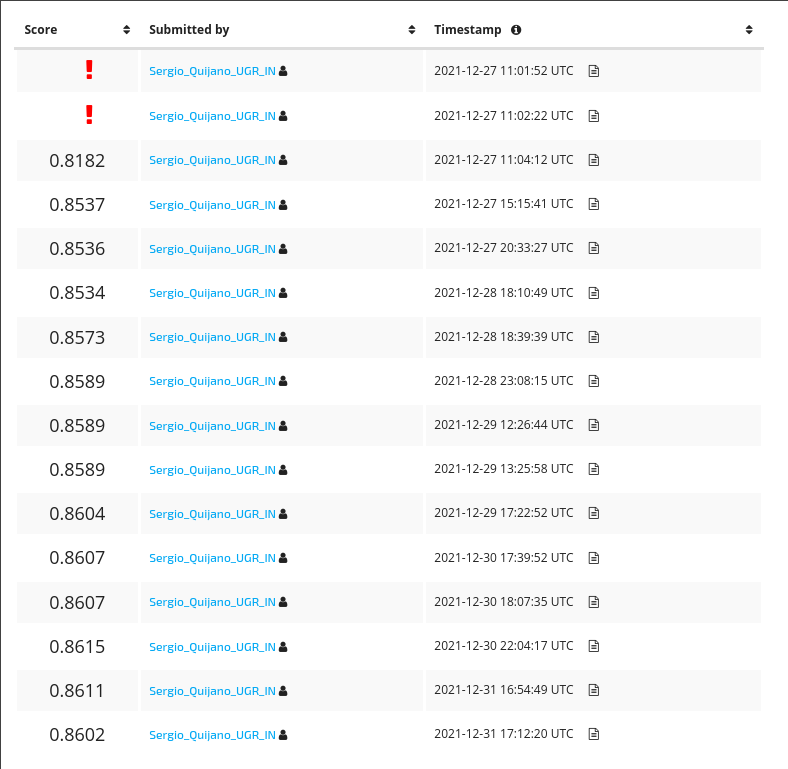
\includegraphics[width = 0.9 \textwidth]{todas_las_propuestas}
    \caption{Tabla de \emph{Driven Data} con la información de todas las propuestas realizadas}
\end{figure}

En la figura anterior podemos ver que las dos primeras entregas no tuvieron \emph{score}. Esto se debe a que subimos los resultados con un formato erróneo.

\pagebreak

\section{Introducción}

\subsection{Descripción del problema}

Según la descripción del problema de \emph{Driven Data} \cite{driven_data_problem_description:online}, debemos calcular la probabilidad de que una persona se vacune de dos tipos de vacunas distintas. Es decir, deberemos calcular dos probabilidades, una por cada tipo de vacuna con la que se trabaja. Las vacunas son para el virus \emph{h1n1} y para la gripe.

Disponemos de 39 columnas. Una de ellas es para el identificador de la persona encuestada (que no usaremos) y dos de ellas son las etiquetas a predecir. Por tanto disponemos de 36 columnas para llevar a cabo la tarea de aprendizaje. Tenemos columnas de tipo numérico y de tipo categórico. Por otro lado, tenemos 26707 ejemplos en nuestra base de datos de entrenamiento.

La métrica a optimizar, y en la que se basará el \emph{ranking} de la competición, será el área bajo la curva ROC. Como tenemos dos etiquetas a predecir, será la media del área bajo la curva ROC para las dos etiquetas por separado.

Por tanto, las propuestas subidas a la plataforma \emph{Driven Data} deberán ser dos valores probabilísticos entre 0 y 1, y no simplemente valores de clasificación binaria $\{0, 1\}$.

Respecto a la plataforma donde se desarrolla la competición, dejan a nuestra disposición dos conjuntos de datos. El conjunto de entrenamiento, etiquetado, y el conjunto de test, sin etiquetar. A partir del conjunto de test deberemos generar la propuesta que subimos a la plataforma. Además, solo dispondremos de 3 propuestas al día. Cuando se realiza una propuesta, se conoce el \emph{score} en test de forma inmediata.

\subsection{Consideraciones iniciales}

En primer lugar, en el fichero que subimos a \emph{PRADO}, el código se encuentra separado en carpetas enumeradas, una carpeta por cada experimento realizado. En cada carpeta se encuentra el \emph{Notebook} conteniendo todo el código empleado, el fichero \lstinline{final_submission.csv} con la propuesta realizada, y dos capturas de pantalla. Una captura con el \emph{score} obtenido en la propuesta, y otra captura que muestra la posición ocupada en el momento de realizar la propuesta.

En segundo lugar, todos los \emph{Notebooks} tendrán una sección inicial con funciones comunes a todo el código. Por ejemplo, funciones para evaluar modelos, para trabajar con \emph{dataframes}, \ldots

En tercer lugar, también tendremos en todos los \emph{Notebooks} una variable \lstinline{RUNNING_ENV}. Cuando es \lstinline{"local"}, indicamos que estamos corriendo el código en nuestra máquina. Cuando es \lstinline{"remote"}, indicamos que estamos corriendo en \emph{Google Colab}. Con esto controlamos diferencias sutiles, como la autorización necesaria en \emph{Google Colab}, o las rutas a la carpeta de datos. Y con ello, evitamos tener que manejar dos bases de código según el entorno en el que estemos corriendo.

Hemos empleado la herramienta \emph{Google Colab} intensamente. Principalmente a la hora de realizar \emph{Hyperparameter Tuning} usando \emph{Cross Validation} para ello. Casi todos los algoritmos han tardado aproximadamente 90 o 120 minutos en terminar su \emph{tuning}, y con la cantidad de algoritmos considerados, hemos llegado a tardar 14h en realizar este proceso de principio a fin. Por tanto, gracias al uso de \emph{Google Colab}, hemos podido dejar esta búsqueda en un segundo plano, para seguir mejorando el código en local, con nuestra máquina sin sobrecargar por este proceso exigente computacionalmente.

En cuarto lugar, subimos también a \emph{PRADO} el archivo \lstinline{pyproject.toml}, en el que definimos todos los paquetes usados para el desarrollo de la práctica. Algunos paquetes pueden no encontrarse en las instalaciones por defecto de entornos de \emph{Data Science} habituales (como pudiera ser \lstinline{conda}). Por tanto, y para permitir reproducir los experimentos independientemente del entorno, especificamos los paquetes empleados en este fichero (que se corresponde al gestor de paquetes \lstinline{poetry}).

En quinto y último lugar, se podrá consultar el código de esta práctica (y de todas las prácticas de la asignatura) en el repositorio de \emph{Github} \url{https://github.com/SergioQuijanoRey/PracticasInteligenciaNegocio}. Este repositorio será público a partir del 7 de enero, momento en el que las prácticas de la asignatura finalizan.

\pagebreak

\section{Desarrollo de los experimentos}

\subsection{Resumen de los experimentos realizados}

En la siguiente tabla mostramos un resumen del desarrollo de los experimentos. El desarrollo de los experimentos se ha realizado de forma incremental. Es decir, hemos partido del experimento anterior, y hemos añadido mejoras o cambios, en la mayoría de los casos no disruptivos. En caso de un cambio de gran calado se indicará en la siguiente tabla. Por lo tanto, la siguiente tabla recoge los cambios de forma incremental.

Por la longitud de las tabla global, separaremos dicha tabla en dos tablas. Una tabla que muestre los resultados obtenidos en la competición, y otra tabla que explique los cambios realizados. Mostramos ambas tablas a continuación:

\begin{table}[H]
\begin{center}
    \begin{tabular}{|p{0.1\linewidth} | p{0.35\linewidth} | p{0.1\linewidth}| p{0.25\linewidth}| p{0.2\linewidth}|}
        \hline
        Propuesta & Fecha y hora (hora española) & Posición ocupada & Score Training & Score Test Driven Data \\

        \hline
        1 & 27/12/2021 12:08 & 793 & - & 0.8182 \\ \hline
        2 & 27/12/2021 16:17 & 398 & 0.8658 & 0.8537 \\ \hline
        3 & 27/12/2021 21:33 & 402 & 0.8426 & 0.8536 \\ \hline
        4 & 28/12/2021 19:12 & 405 & 0.85966 & 0.8534 \\ \hline
        5 & 28/12/2021 19:40 & 339 & 0.8630 & 0.8573 \\ \hline
        6 & 29/12/2021 00:09 & 305 & 0.8823 & 0.8589 \\ \hline
        7 & 29/12/2021 13:27 & 305 & 0.8646 & 0.8589 \\ \hline
        8 & 29/12/2021 14:26 & 305 & 0.8648 & 0.8589 \\ \hline
        9 & 29/12/2021 18:25 & 248 & 0.8641 & 0.8604 \\ \hline
    \end{tabular}
\end{center}
    \caption{Resumen de los resultados logrados con los cambios incrementales a lo largo de la práctica}
    \label{resumen_resultados:tabla}
\end{table}

\begin{landscape}
\begin{table}[t]
\begin{center}
    \begin{tabular}{|p{0.1\linewidth} | p{0.3\linewidth} | p{0.3\linewidth}| p{0.3\linewidth}|}
        \hline
        Nombre Propuesta & Descripción preprocesado & Descripción Algoritmo & Configuración de parámetros \\ \hline
        1 & Nos quedamos solo con las variables numéricas, imputamos los missing values usando la mediana & Regresión logística, entrenando dos modelos para las dos variables objetivo & C = 1, regularización l2 \\ \hline
        2 & Imputamos missing values con la mediana. Normalizamos a media 0 y desviación 1. Nos quedamos con las variables categóricas, que transformamos a numéricas usando \emph{one hot encoding} & Añadimos cross validation. Decidimos usar AdaBoost. Añadimos la evaluación del modelo sobre el conjunto de validación & lr = 0.5, n\_estimators = 200 \\ \hline
        3 & Imputamos missing values con un estimador en base a las otras variables. Usamos Smote+TomekLinks & Volvemos a hacer CV y tomamos los mejores parámetros & lr = 0.75 n\_estimatos = 200 \\ \hline
        4 & Borramos SMOTE + TomekLinks, cacheamos el pre-procesado de datos para poder hacer iteraciones más rápidas & Añadimos CatBoost y hacemos CV para seleccionar los mejores hiperparámetros & lr = 0.5, iterations = 20, depth = 4 \\ \hline
        5 & Entrenamos sobre todo el conjunto de datos tras entrenar y evaluar en validación & Catboost al que hemos cambiado manualmente los parámetros & lr = 0.5, iterations = 40, depth = 4 \\ \hline
        6 & - & Ajustamos CV para todos los modelos, incluido Random Forest. Sigue siendo el mejor Catboost & lr = 0.25, iterations = 80, depth = 4 \\ \hline
        7 & - & Ensemble con los cuatro algoritmos, con los mejores parámetros que hemos encontrado & Logistic: penalty = "l2", C = 0.05 ; Adaboost: n\_estimators = 200, learning\_rate = 0.5 ; Catboost: iterations=80, learning\_rate=0.25, depth=4 ; Random Forest:     n\_estimators = 200, criterion = "entropy", min\_samples\_split = 4, min\_samples\_leaf = 3 \\ \hline
        8 & - & Ponderamos el ensemble con los resultados de los modelos individuales, en validación, aplicando softmax & - \\ \hline
        9 & Además del borrado de outliers que teníamos, añado IsolationForest para borrar outliers & Aplicamos correctamente el ensemble (estábamos re-entrenando con un Catboost simple) & - \\ \hline
    \end{tabular}
\end{center}
    \caption{Resumen de los cambios incrementales realizados a lo largo de la práctica}
    \label{resumen_cambios:tabla}
\end{table}
\end{landscape}

Notar que en \customcite{resumen_resultados:tabla}, en la primera propuesta, no tenemos resultados de \emph{training}. Esto se debe a que, como comentaremos más adelante, en esta primera propuesta todavía no habíamos desarrollado un método de evaluación de los resultados, y por tanto no tuvimos disponible esa métrica. Y notar también que, en \customcite{resumen_cambios:tabla}, cuando no hacemos cambios o bien en los algoritmos o bien en el tratamiento de los datos, indicamos con un \entrecomillado{$-$} dicha ausencia de cambios, evitando así ser excesivamente repetitivos.

Con todo esto, pasamos a desarrollar, propuesta a propuesta, el trabajo desarrollado.

\pagebreak

\subsection{Experimento 1}

En este primer experimento, escribimos el mínimo código para poder hacer una \emph{submission} y familiarizarnos así con la plataforma. Por tanto, y como se puede apreciar en \customcite{resumen_resultados:tabla}, no tenemos información sobre el rendimiento de nuestro modelo en \emph{training}.

Parte de nuestro código lo basamos en el código que \emph{Driven Data} muestra como \emph{benchmark} \cite{datadriven_example:online}, aunque gran parte del código la tomamos de una plantilla nuestra, preparada con las tareas más repetitivas de todo proyecto de \emph{Data Science}. En concreto, tomamos el modelo propuesto en el ejemplo, y el código para realizar la propuesta.

El pre-procesado de los datos es muy básico:

\begin{enumerate}
    \item Empezamos borrando la columna \lstinline{"respondent_id"}. No nos hace falta, pues el \lstinline{dataframe} ya guarda en su estado interno un identificador para las filas
    \item Filtramos todas las variables categóricas, solo nos quedamos con las numéricas
    \item Separamos el conjunto de entrenamiento en entrenamiento (80\%) y validación (20\%)
    \item Imputamos los \emph{missing values} usando la mediana
\end{enumerate}

En este pre-procesado, y en todos los siguientes, cuando realizamos una transformación sobre el conjunto de entrenamiento con parámetros que se aprenden, se aplicará en validación y test con dichos parámetros, aprendidos en entrenamiento. Si aprendiésemos dichos parámetros sobre todo el conjunto de datos (\emph{training}, validación y test juntos) estaríamos cometiendo \emph{data snooping}.

A la hora de separar en \emph{training} y \emph{validation}, usamos estratificación por la etiqueta de salida. Como tenemos dos etiquetas, las combinamos en una sola, estratificamos usando esa etiqueta combinada, y deshacemos el combinado de etiquetas.

El modelo aplicado es muy básico: dos modelos de regresión logística. En este caso, y en todos los posteriores, entrenaremos dos modelos del mismo tipo para clasificar las dos etiquetas. Esto lo haremos cómodamente con la clase \lstinline{MultiOutputClassifier}. De ahora en adelante, este detalle técnico lo omitiremos y hablaremos directamente de modelos, entendiendo por ello lo que aquí detallamos.

Es en este experimento en el que realizamos dos propuestas fallidas, como muestra \customcite{resumen_resultados:tabla}.

Los resultados se muestran en las siguientes figura:

\begin{figure}[H]
    \centering

    \begin{subfigure}[b]{0.45 \textwidth}
        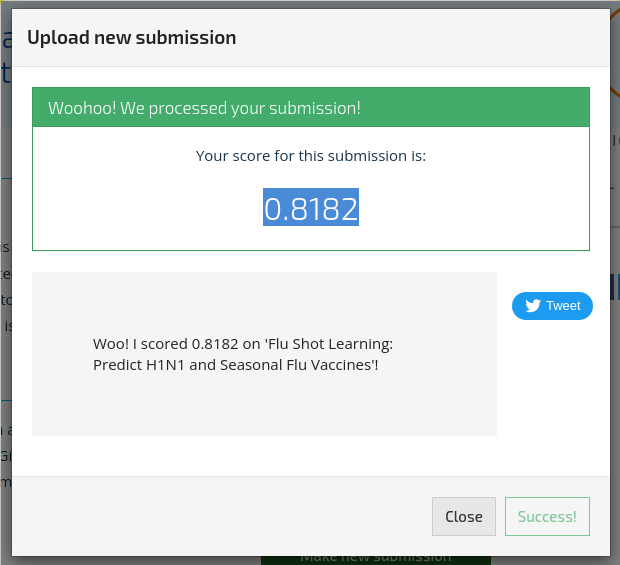
\includegraphics[width = 0.9 \textwidth]{../Notebook01/27-12-2021::12:08:09.png}
        \caption{Score obtenida en la \emph{submission}}
    \end{subfigure}
    \begin{subfigure}[b]{0.45 \textwidth}
        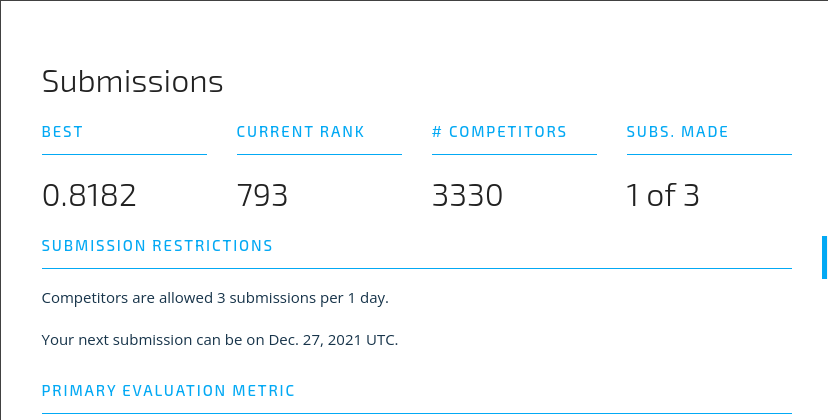
\includegraphics[width = 0.9 \textwidth]{../Notebook01/27-12-2021::12:08:42.png}
        \caption{Posición de ese momento en la competición}
    \end{subfigure}

    \caption{Resultados obtenidos tras hacer la \emph{submission} en la plataforma \emph{online}}
\end{figure}

\pagebreak

\subsection{Experimento 2}

El pre-procesado en este experimento es:

\begin{enumerate}
    \item Seguimos imputando los \emph{missing values} con la mediana
    \item Normalizamos el conjunto de datos a media 0 y desviación típica 1
    \item En vez de eliminar las variables numéricas, las pasamos a numéricas con \emph{one hot enconding} y las consideramos en nuestro conjunto de entrenamiento
\end{enumerate}

Además de ese pre-procesado de los datos, añadimos el modelo \emph{Adaboost}. Escribimos un \emph{GridSearch} propio para hacer \emph{Hyper Parameter Tuning}. Con esto nos referimos a que especificamos los conjuntos de parámetros manualmente, así como el bucle en que evaluamos con \emph{10-fold Cross Validation}. Con esto tenemos un mayor control en este proceso que puede ser muy largo. Por ejemplo, podemos parar la búsqueda en la mitad del proceso, y tomar el mejor parámetro encontrado hasta el momento. O definir los \emph{logs} que queremos mostrar durante el proceso. Esto no lo podíamos hacer con la funcionalidad correspondientes de \lstinline{sklearn}, y al no suponer mucho código, lo implementamos nosotros para resolver nuestras necesidades.

Aplicamos dicha búsqueda a los dos modelos que hemos tratado hasta ahora. Empleamos \emph{Adaboost} por dar mejores resultados.

Además, añadimos la evaluación del modelo. Para ello, llamamos a la función propia \lstinline{evaluate_model}, en la que calculamos algunas métricas adicionales.

Todavía no hemos implementado el re-entrenamiento sobre todo el conjunto de datos, así que la \emph{submission} se realiza con el modelo entrenado en un subconjunto de los datos iniciales.

Los resultados se muestran en las siguiente figura:

\begin{figure}[H]
    \centering

    \begin{subfigure}[b]{0.45 \textwidth}
        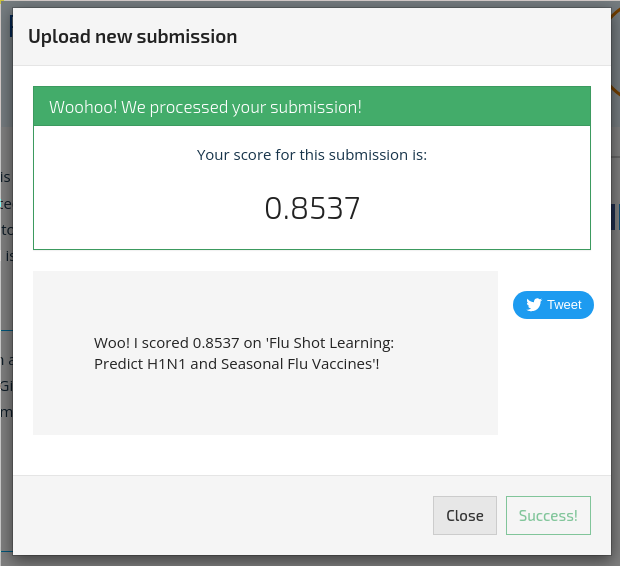
\includegraphics[width = 0.9 \textwidth]{../Notebook02/27-12-2021::16:16:34.png}
        \caption{Score obtenida en la \emph{submission}}
    \end{subfigure}
    \begin{subfigure}[b]{0.45 \textwidth}
        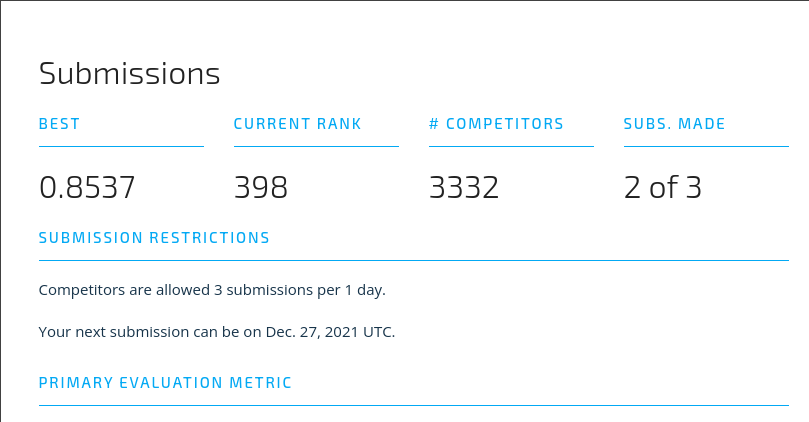
\includegraphics[width = 0.9 \textwidth]{../Notebook02/27-12-2021::16:16:54.png}
        \caption{Posición de ese momento en la competición}
    \end{subfigure}

    \caption{Resultados obtenidos tras hacer la \emph{submission} en la plataforma \emph{online}}
\end{figure}

\pagebreak

\subsection{Experimento 3}

Los cambios en el pre-procesado de datos son:

\begin{itemize}
    \item En vez de imputar \emph{missing values} usando la mediana, usamos predictores en el resto de variables
    \item
\end{itemize}

% Bibliografia
\bibliography{./References}
\bibliographystyle{ieeetr}

\end{document}
